%%%%%%%%%%%%%%%%%%%%%%%%%%%%%%%%%%%%%%%%%
% Journal Article
% LaTeX Template
% Version 1.4 (15/5/16)
%
% This template has been downloaded from:
% http://www.LaTeXTemplates.com
%
% Original author:
% Frits Wenneker (http://www.howtotex.com) with extensive modifications by
% Vel (vel@LaTeXTemplates.com)
%
% License:
% CC BY-NC-SA 3.0 (http://creativecommons.org/licenses/by-nc-sa/3.0/)
%
%%%%%%%%%%%%%%%%%%%%%%%%%%%%%%%%%%%%%%%%%

%----------------------------------------------------------------------------------------
%	PACKAGES AND OTHER DOCUMENT CONFIGURATIONS
%----------------------------------------------------------------------------------------

\documentclass[twoside,twocolumn]{article}

\usepackage{blindtext} % Package to generate dummy text throughout this template 

\usepackage{hyperref}
\hypersetup{
    colorlinks=true,
    linkcolor=blue,
    filecolor=magenta,      
    urlcolor=cyan,
}

\usepackage[sc]{mathpazo} % Use the Palatino font
\usepackage[T1]{fontenc} % Use 8-bit encoding that has 256 glyphs
\linespread{1.05} % Line spacing - Palatino needs more space between lines
\usepackage{microtype} % Slightly tweak font spacing for aesthetics
\usepackage[utf8]{inputenc}

\usepackage[portuguese]{babel} % Language hyphenation and typographical rules

\usepackage[hmarginratio=1:1,top=32mm,columnsep=20pt]{geometry} % Document margins
\usepackage[hang, small,labelfont=bf,up,textfont=it,up]{caption} % Custom captions under/above floats in tables or figures
\usepackage{booktabs} % Horizontal rules in tables

\usepackage{lettrine} % The lettrine is the first enlarged letter at the beginning of the text
\usepackage{float}
\usepackage{enumitem} % Customized lists
\setlist[itemize]{noitemsep} % Make itemize lists more compact

\usepackage{abstract} % Allows abstract customization
\renewcommand{\abstractnamefont}{\normalfont\bfseries} % Set the "Abstract" text to bold
\renewcommand{\abstracttextfont}{\normalfont\small\itshape} % Set the abstract itself to small italic text
%\usepackage[shortlabels]{enumitem}
\usepackage{enumitem}
\usepackage{titlesec} % Allows customization of titles
\renewcommand\thesection{\Roman{section}} % Roman numerals for the sections
\renewcommand\thesubsection{\roman{subsection}} % roman numerals for subsections
\titleformat{\section}[block]{\large\scshape\centering}{\thesection.}{1em}{} % Change the look of the section titles
\titleformat{\subsection}[block]{\large}{\thesubsection.}{1em}{} % Change the look of the section titles

\usepackage{fancyhdr} % Headers and footers
\pagestyle{fancy} % All pages have headers and footers
\fancyhead{} % Blank out the default header
\fancyfoot{} % Blank out the default footer
\fancyhead[C]{MO443 $\bullet$ Maio 2019 $\bullet$ Relatório 02} % Custom header text
\fancyfoot[RO,LE]{\thepage} % Custom footer text

\usepackage{titling} % Customizing the title section

\usepackage{hyperref} % For hyperlinks in the PDF

\usepackage{graphicx}
\usepackage{subfigure}

\usepackage{mathtools}
\DeclarePairedDelimiter\floor{\lfloor}{\rfloor}
%----------------------------------------------------------------------------------------
%	TITLE SECTION
%----------------------------------------------------------------------------------------

\setlength{\droptitle}{-4\baselineskip} % Move the title up

\pretitle{\begin{center}\Huge\bfseries} % Article title formatting
\posttitle{\end{center}} % Article title closing formatting
\title{Relatório - Trabalho 02 \\ \Large MO443 - Introdução ao Processamento de Imagem Digital} %
%\subtitle{qsdqwdqwd} %Article title
\author{%
\textsc{Vinicius Teixeira de Melo - RA: 230223} \\[1ex] % Your name
\normalsize Universidade Estadual de Campinas \\ % Your institution
\normalsize \href{mailto:viniciusteixeira@liv.ic.unicamp.br}{viniciusteixeira@liv.ic.unicamp.br} % Your email address
%\and % Uncomment if 2 authors are required, duplicate these 4 lines if more
%\textsc{Jane Smith}\thanks{Corresponding author} \\[1ex] % Second author's name
%\normalsize University of Utah \\ % Second author's institution
%\normalsize \href{mailto:jane@smith.com}{jane@smith.com} % Second author's email address
}
\date{\today} % Leave empty to omit a date
\renewcommand{\maketitlehookd}{%
%\begin{abstract}
%\noindent \blindtext % Dummy abstract text - replace \blindtext with your abstract text
%\end{abstract}
}

%----------------------------------------------------------------------------------------

\begin{document}

% Print the title
\maketitle

%----------------------------------------------------------------------------------------
%	ARTICLE CONTENTS
%----------------------------------------------------------------------------------------

\section{Especificação do Problema}

O objetivo deste trabalho é implementar duas técnicas de quantização de cores, definidas como técnicas de pontilhado que visam reduzir a quantidade de cores utilizadas para exibir uma imagem, procurando manter uma boa percepção por parte do usuário.

O trabalho é dividido em duas partes. A primeira é escrever uma função para alterar os níveis de cinza $[f_{min} \dots f_{max}]$ de uma imagem $f(x,y)$ por meio das técnicas de pontilhado (\textit{half-toning}) ordenado, produzindo uma imagem $g(x,y)$.

O algoritmo de pontilhado ordenado utiliza um conjunto de padrões formados por pontos pretos e brancos. O conjunto de dez padrões, ilustrados na Figura~\ref{padroes}, pode ser representado por meio da matriz $M_{3x3}$ a seguir:

\vspace{0.5cm}

$M_{3x3} = $ \begin{tabular}{|c|c|c|}
\hline
6 & 8 & 4 \\ \hline
1 & 0 & 3 \\ \hline
5 & 2 & 7 \\ \hline
\end{tabular}

\begin{figure}[H]
\begin{center}
	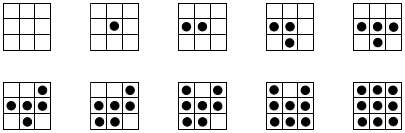
\includegraphics[height=2cm]{figures/padroes.png}
\caption{Dez padrões de 3 x 3 pixels.} \label{padroes}
\end{center}
\end{figure}

Os valores das células da matriz podem ser utilizados como limiares. Se o valor do pixel (normalizado entre 0 e 9) for menor do que o número correspondente à célula da matriz, o pixel será substituído pelo valor preto, caso contrário, será substituído pelo valor branco.

Uma outra máscara, conhecida como matriz de pontilhado ordenado de Bayer, é dada por

\vspace{0.3cm}

$M_{4x4} = $ \begin{tabular}{|c|c|c|c|}
\hline
0  & 12 & 3  & 15 \\ \hline
8  & 4  & 11 & 7  \\ \hline
2  & 14 & 1  & 13 \\ \hline
10 & 6  & 9  & 5  \\ \hline
\end{tabular}

\vspace{0.3cm}

A segunda parte do trabalho é aplicar o algoritmo de pontilhado por difusão de erro também transforma a imagem original em uma imagem contendo apenas os valores preto e branco, entretanto, leva em consideração os valores ao redor de cada pixel. A técnica de pontilhado por difusão de erro de \textit{Floyd-Steinberg} é resumida a seguir:

\begin{enumerate}
	\item percorra todos os pixels da imagem, segundo uma ordem pré-definida;
	\item para cada pixel, se seu valor for maior do que 128, troque-o para 255 (branco). Caso contrário, troque-o para 0 (preto). Armazene o erro, ou seja, a diferença entre o valor exato do pixel e o valor aproximado.
	\item distribua o erro aos pixels adjacentes, da seguinte forma (Figura~\ref{distribuicao}):
		\begin{enumerate}
			\item adicione $\dfrac{7}{16}$ do erro ao pixel localizado à direita.
			\item adicione $\dfrac{3}{16}$ do erro ao pixel localizado abaixo e à esquerda.
			\item adicione $\dfrac{5}{16}$ do erro ao pixel localizado abaixo.
			\item adicione $\dfrac{1}{16}$ do erro ao pixel localizado abaixo e à direita.
		\end{enumerate}
\end{enumerate}

\begin{figure}[H]
\begin{center}
	\begin{tabular}{|c|c|c|}
\hline
     &        &      \\ \hline
     & f(x,y) & 7/16 \\ \hline
3/16 & 5/16   & 1/16 \\ \hline
\end{tabular}
\caption{Distribuição de erro na técnica de pontilhado com difusão de erro de \textit{Floyd-Steinberg}.} \label{distribuicao}
\end{center}
\end{figure}

A ordem na qual a imagem é percorrida pode produzir resultados diferentes no processo de dithering. A varredura da esquerda para a direita (Figura~\ref{varredura}(a)) pode gerar padrões indesejados ou a impressão de uma certa direcionalidade na imagem resultante. Para evitar esses efeitos, uma alternativa é modificar a direção de varredura a cada linha (Figura~\ref{varredura}(b)).

\begin{figure}[H]
\begin{center}
	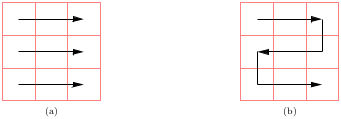
\includegraphics[height=2cm]{figures/varredura.png}
\caption{Formas de varredura da imagem.} \label{varredura}
\end{center}
\end{figure}

Portanto, o trabalho é a aplicação dessas duas técnicas de pontilhado.

%------------------------------------------------

\section{Entrada de Dados}

O código fonte criado para a execução de todas as tarefas está no notebook \textbf{Trabalho 02.ipynb}. O código foi criado para aceitar imagens em tons de cinza do tipo PGM (\textit{Portable GrayMap}).

Para executar o notebook, basta iniciar o ambiente \textit{Jupyter Notebook}, abrir o notebook \textbf{Trabalho 02.ipynb} e executar as células em ordem. Todo o algoritmo foi implementado na linguagem Python na versão 3.6.

As imagens de entrada utilizadas nos testes do algoritmo foram retiradas da página do prof. Hélio Pedrini: \href{http://www.ic.unicamp.br/~helio/imagens_pgm/}{Imagens}. Na pasta \textbf{imgs/} estão as três imagens monocromáticas utilizadas nos testes: \textbf{baboon.pgm}, \textbf{fiducial.pgm} e \textbf{monarch.pgm}. As dimensões das imagens de entrada utilizadas são 512x512, 640x480 e 768x512, respectivamente.

\begin{figure}[H]
\begin{center}
	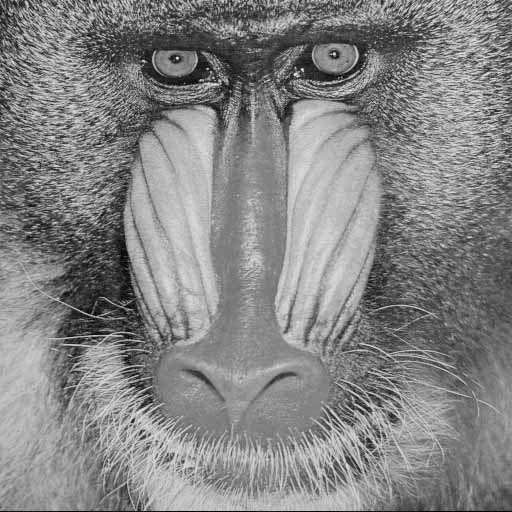
\includegraphics[height=3cm]{figures/baboon.png}
\caption{baboon.pgm} \label{gdimotes}
\end{center}
\end{figure}

\begin{figure}[H]
\begin{center}
	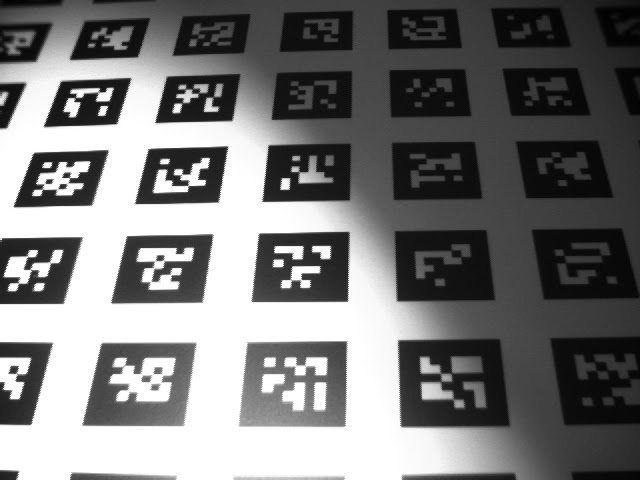
\includegraphics[height=3cm]{figures/fiducial.png}
\caption{fiducial.pgm} \label{gdimotes}
\end{center}
\end{figure}

\begin{figure}[H]
\begin{center}
	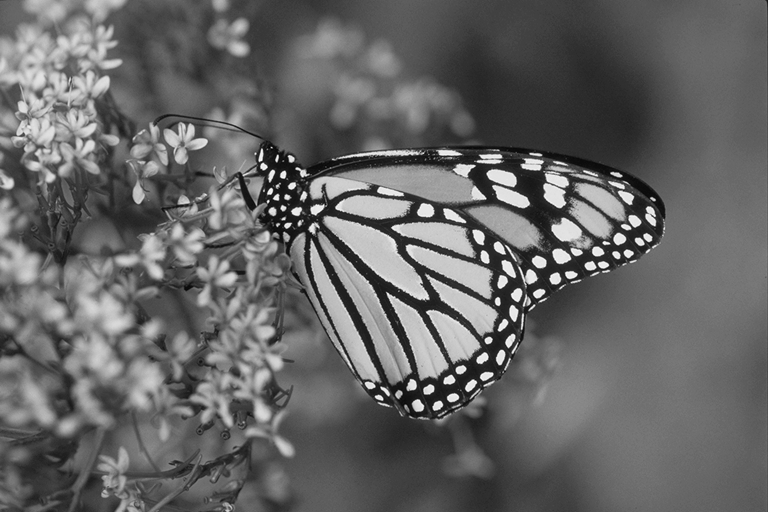
\includegraphics[height=3cm]{figures/monarch.png}
\caption{monarch.pgm} \label{gdimotes}
\end{center}
\end{figure}

%------------------------------------------------

\section{Dependências e Códigos}

As bibliotecas utilizadas neste trabalho foram:

\begin{table}[H]
\begin{tabular}{|l|l|}
\hline
\textbf{Biblioteca} & \textbf{Versão} \\ \hline
numpy               & 1.16.2          \\ \hline
cv2                 & 3.4.2           \\ \hline
matplotlib          & 3.0.3           \\ \hline
warnings            & 2.1             \\ \hline
\end{tabular}
\end{table}

A leitura das imagens foi realizada utilizando uma função do \textbf{opencv} \cite{b1} chamada \textbf{imread()}, a qual necessitou de uma constante do próprio \textbf{opencv} para que a imagem ficassem apenas com o canal de escala de cinza, essa constante é denominada \textbf{IMREAD\_GRAYSCALE}.

As máscaras foram gerados manualmente através da função \textbf{numpy.array()}. A função para normalizar os níveis de cinza foi feita aplicando a fórmula de mudança de base descrita a seguir:

\begin{equation*}
	g(x) = \left(\dfrac{g_{max} - g_{min}}{f_{max} - f_{min}}\right) (f(x) - f_{min}) + g_{min}
\end{equation*}

A função de aplicação da técnica de pontilhamento \textit{half-toning} foi feita manualmente, aplicando primeiramente a normalização de intensidade dos pixels, e depois o preenchimento da nova imagem com base nos valores que eram obtidos através da utilização da máscara como \textit{threshold}.

As funções para a aplicação da técnica de pontilhamento com difusão de erro de \textit{Floyd-Steinberg} também foram feitas manualmente, a qual a primeira, \textbf{floyd\_steinberg\_order1}, percorre a imagem como mostrado na Figura~\ref{varredura}(a) e a segunda, \textbf{floyd\_steinberg\_order2}, percorre a imagem como mostrado na Figura~\ref{varredura}(b).

%------------------------------------------------

\section{Fundamentação}

\subsection{Pontilhado Ordenado}

Também conhecido como \textit{Halftone} (meio-tom), o pontilhado ordenado é uma técnica de processamento de imagens que emprega padrões de pontos pretos ou brancos para reduzir o número de níveis de cinza de uma representação. Defivo ao fato do sistema visual humano atenuar a distinção entre os pontos com tons diferentes, os padrões de pontos pretos e brancos produzem um efeito visual como se a imagem fosse composto por mais tons de cinza \cite{b4}.

No caso de uma máscara $3x3$, cada conjunto de níveis de cinza é representado por um padrão $3x3$ de pontos brancos ou pretos. Uma área de $3x3$ pixels cheia de pontos pretos é uma aproximação de um nível de cinza preto (ou 0). De forma análoga, uma área $3x3$ de pontos totalmente brancos será uma aproximação do branco em uma escala de nível de cinza (ou 9). Os demais padrões intermediários entre $]0,255[$ serão re-escalados para o intervalo $[0,9]$, conforme ilustrado na Figura~\ref{escalas}.

\begin{figure}[H]
\begin{center}
	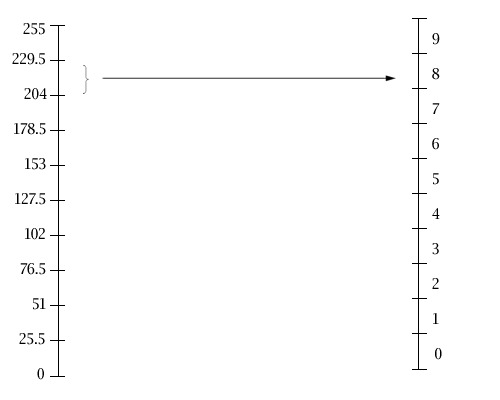
\includegraphics[scale=.009]{figures/escalas.jpg}
\caption{Transformação de escala com uma máscara $3x3$.} \label{escalas}
\end{center}
\end{figure}

É possível notar que utilizamos nove limiares (\textit{threshold}) para a sub-codificação: o intervalo $[0,25.5[$ é truncado para $0$, $[25.5,51[$ é truncado para $1$, $[51,76.5[$ para $2$, e assim por diante. Assim, cada pixel na imagem de entrada irá corresponder a um padrão de $3x3$ pixels na imagem gerada. Desta forma, a resolução espacial será reduzida a $33\%$ da resolução espacial original. Isto é, antes da substituição de cada pixel pela máscara devemos reduzir em $\frac{1}{3}$ as dimensões da imagem para que o resultado tenha o mesmo tamanho da original \cite{b4}.

\subsection{Pontilhado com Difusão de Erro}

Pontilhado com difusão de erro é uma técnica de \textit{halftone} que procura distribuir a diferença entre o valor exato de cada pixel e seu valor aproximado a um conjunto de pixels adjacentes. Diversas técnicas foram desenvolvidas com esta proposta, sendo o algoritmo de Floyd-Steinberg o primeiro desenvolvido utilizando esta abordagem \cite{b5}.

O algoritmo varre a imagem da esquerda para a direita, de cima para baixo, quantificando os valores de pixel um por um. O erro de quantização é transferido para os pixels vizinhos, embora não afete os pixels que já foram quantizados. Assim, se um número de pixels tiver sido arredondado para baixo, torna-se mais provável que o próximo pixel seja arredondado para cima, de modo que, em média, o erro de quantização seja próximo de zero.

Os coeficientes de difusão têm a propriedade de que, se os valores de pixel originais estiverem exatamente na metade entre as cores disponíveis mais próximas, o resultado pontilhado será um padrão de tabuleiro de damas. Por exemplo, $50\%$ de dados em cinza podem ser pontilhados como um padrão quadriculado preto e branco. Para um pontilhamento ótimo, a contagem de erros de quantização deve ter precisão suficiente para evitar que os erros de arredondamento afetem o resultado \cite{b6}.

%------------------------------------------------

\section{Saída de Dados}

Os imagens resultantes foram salvas dentro da pasta \textbf{resultados/} utilizando uma função da biblioteca \textbf{opencv} chamada \textbf{cv2.imwrite()} \cite{b1}.

O formato dos nomes de saída estão da seguinte forma: para a técnica de pontilhado ordenado o padrão é o nome da imagem de entrada (\textit{baboon}, \textit{fiducial} e \textit{monarch}) concatenado com o nome da máscara considerada para a aplicação da função sobre ela; para a técnica de pontilhado com difusão de erros são gerados duas imagens de saída para cada imagem de entrada, uma para cada forma de percorrer a imagem.

%------------------------------------------------

\section{Resultados e Discuções}

Os resultados obtidos com a aplicação da técnica de pontilhado ordenado (\textit{halg-toning}) estão a seguir:

\begin{figure}[H]
\begin{center}
	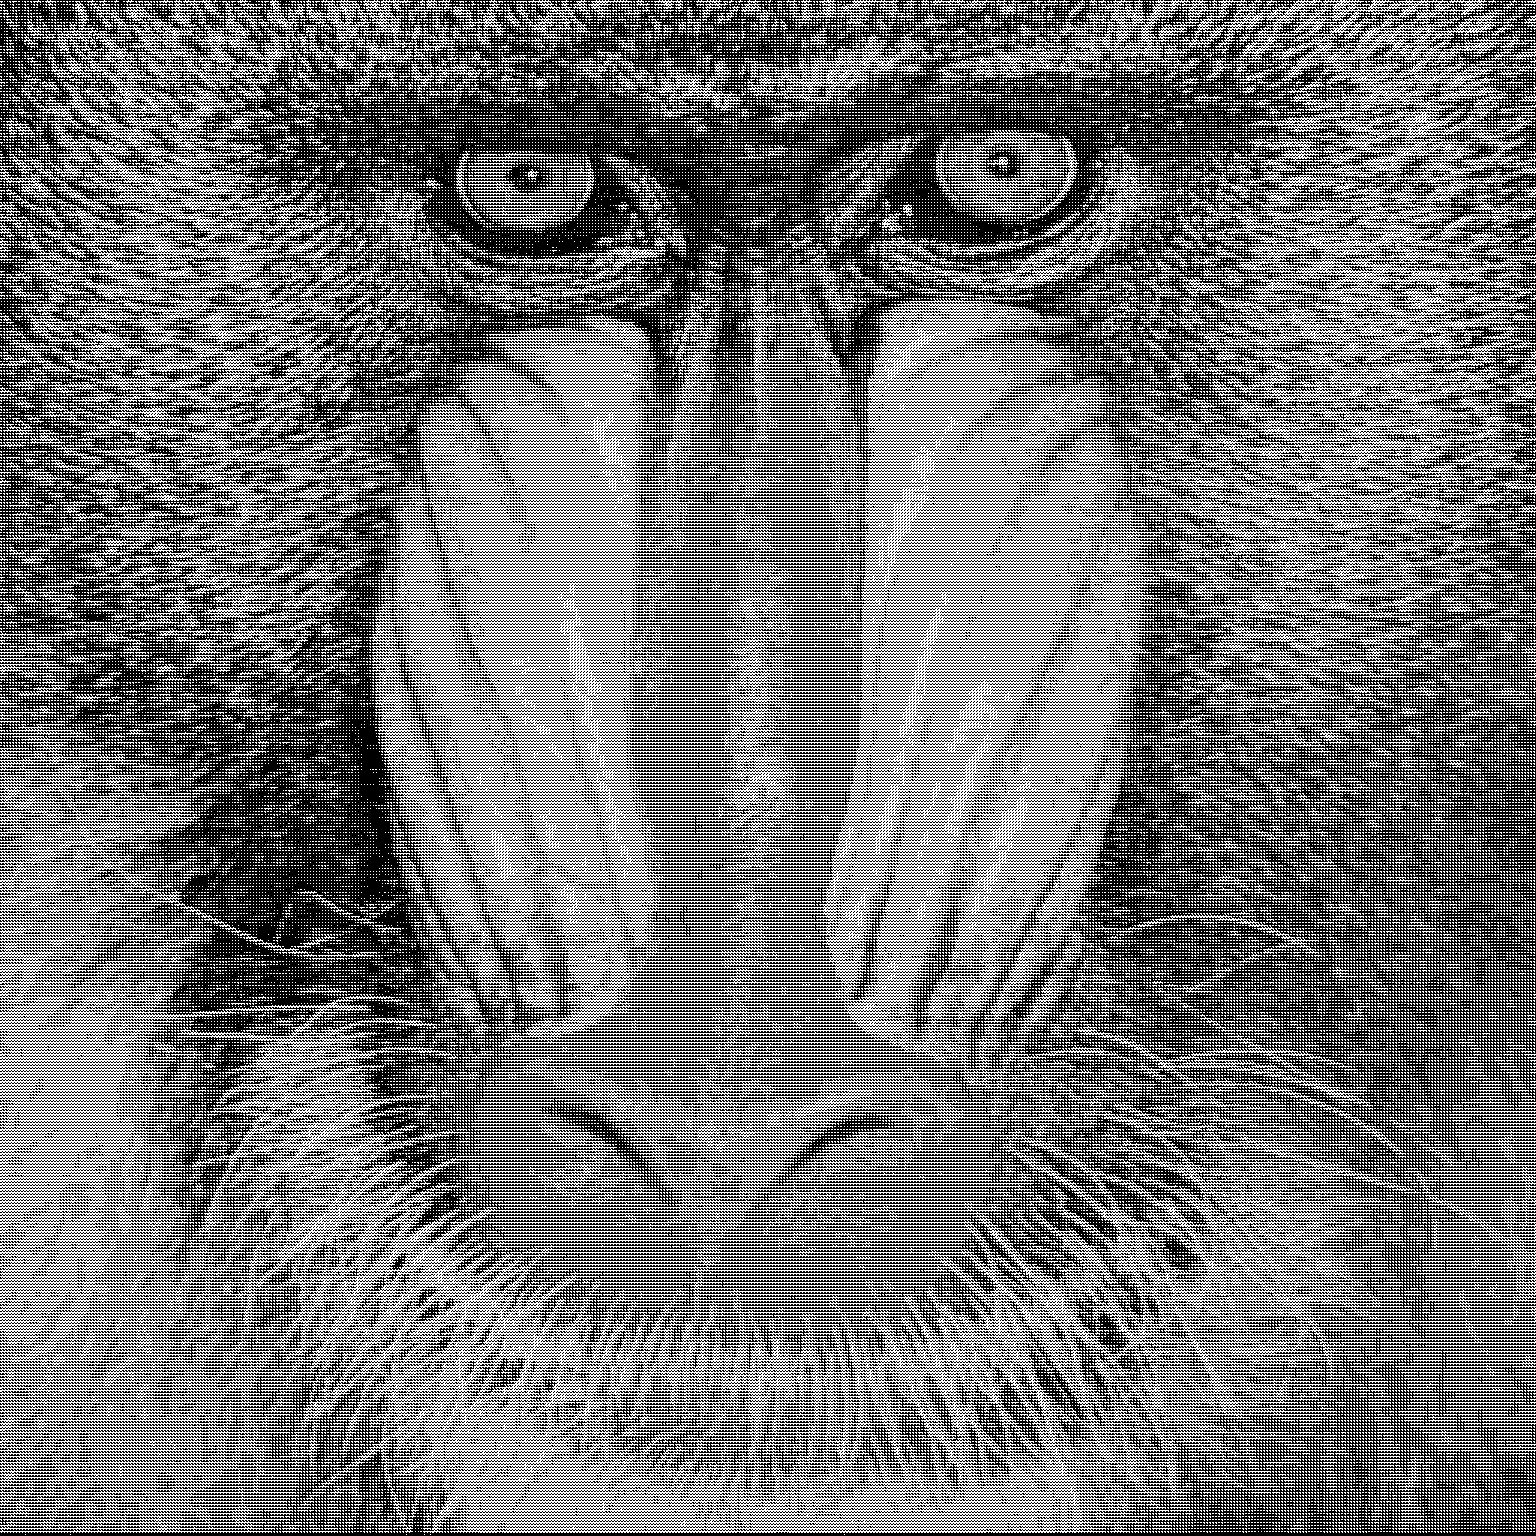
\includegraphics[height=4cm]{figures/baboon_m33.png}
	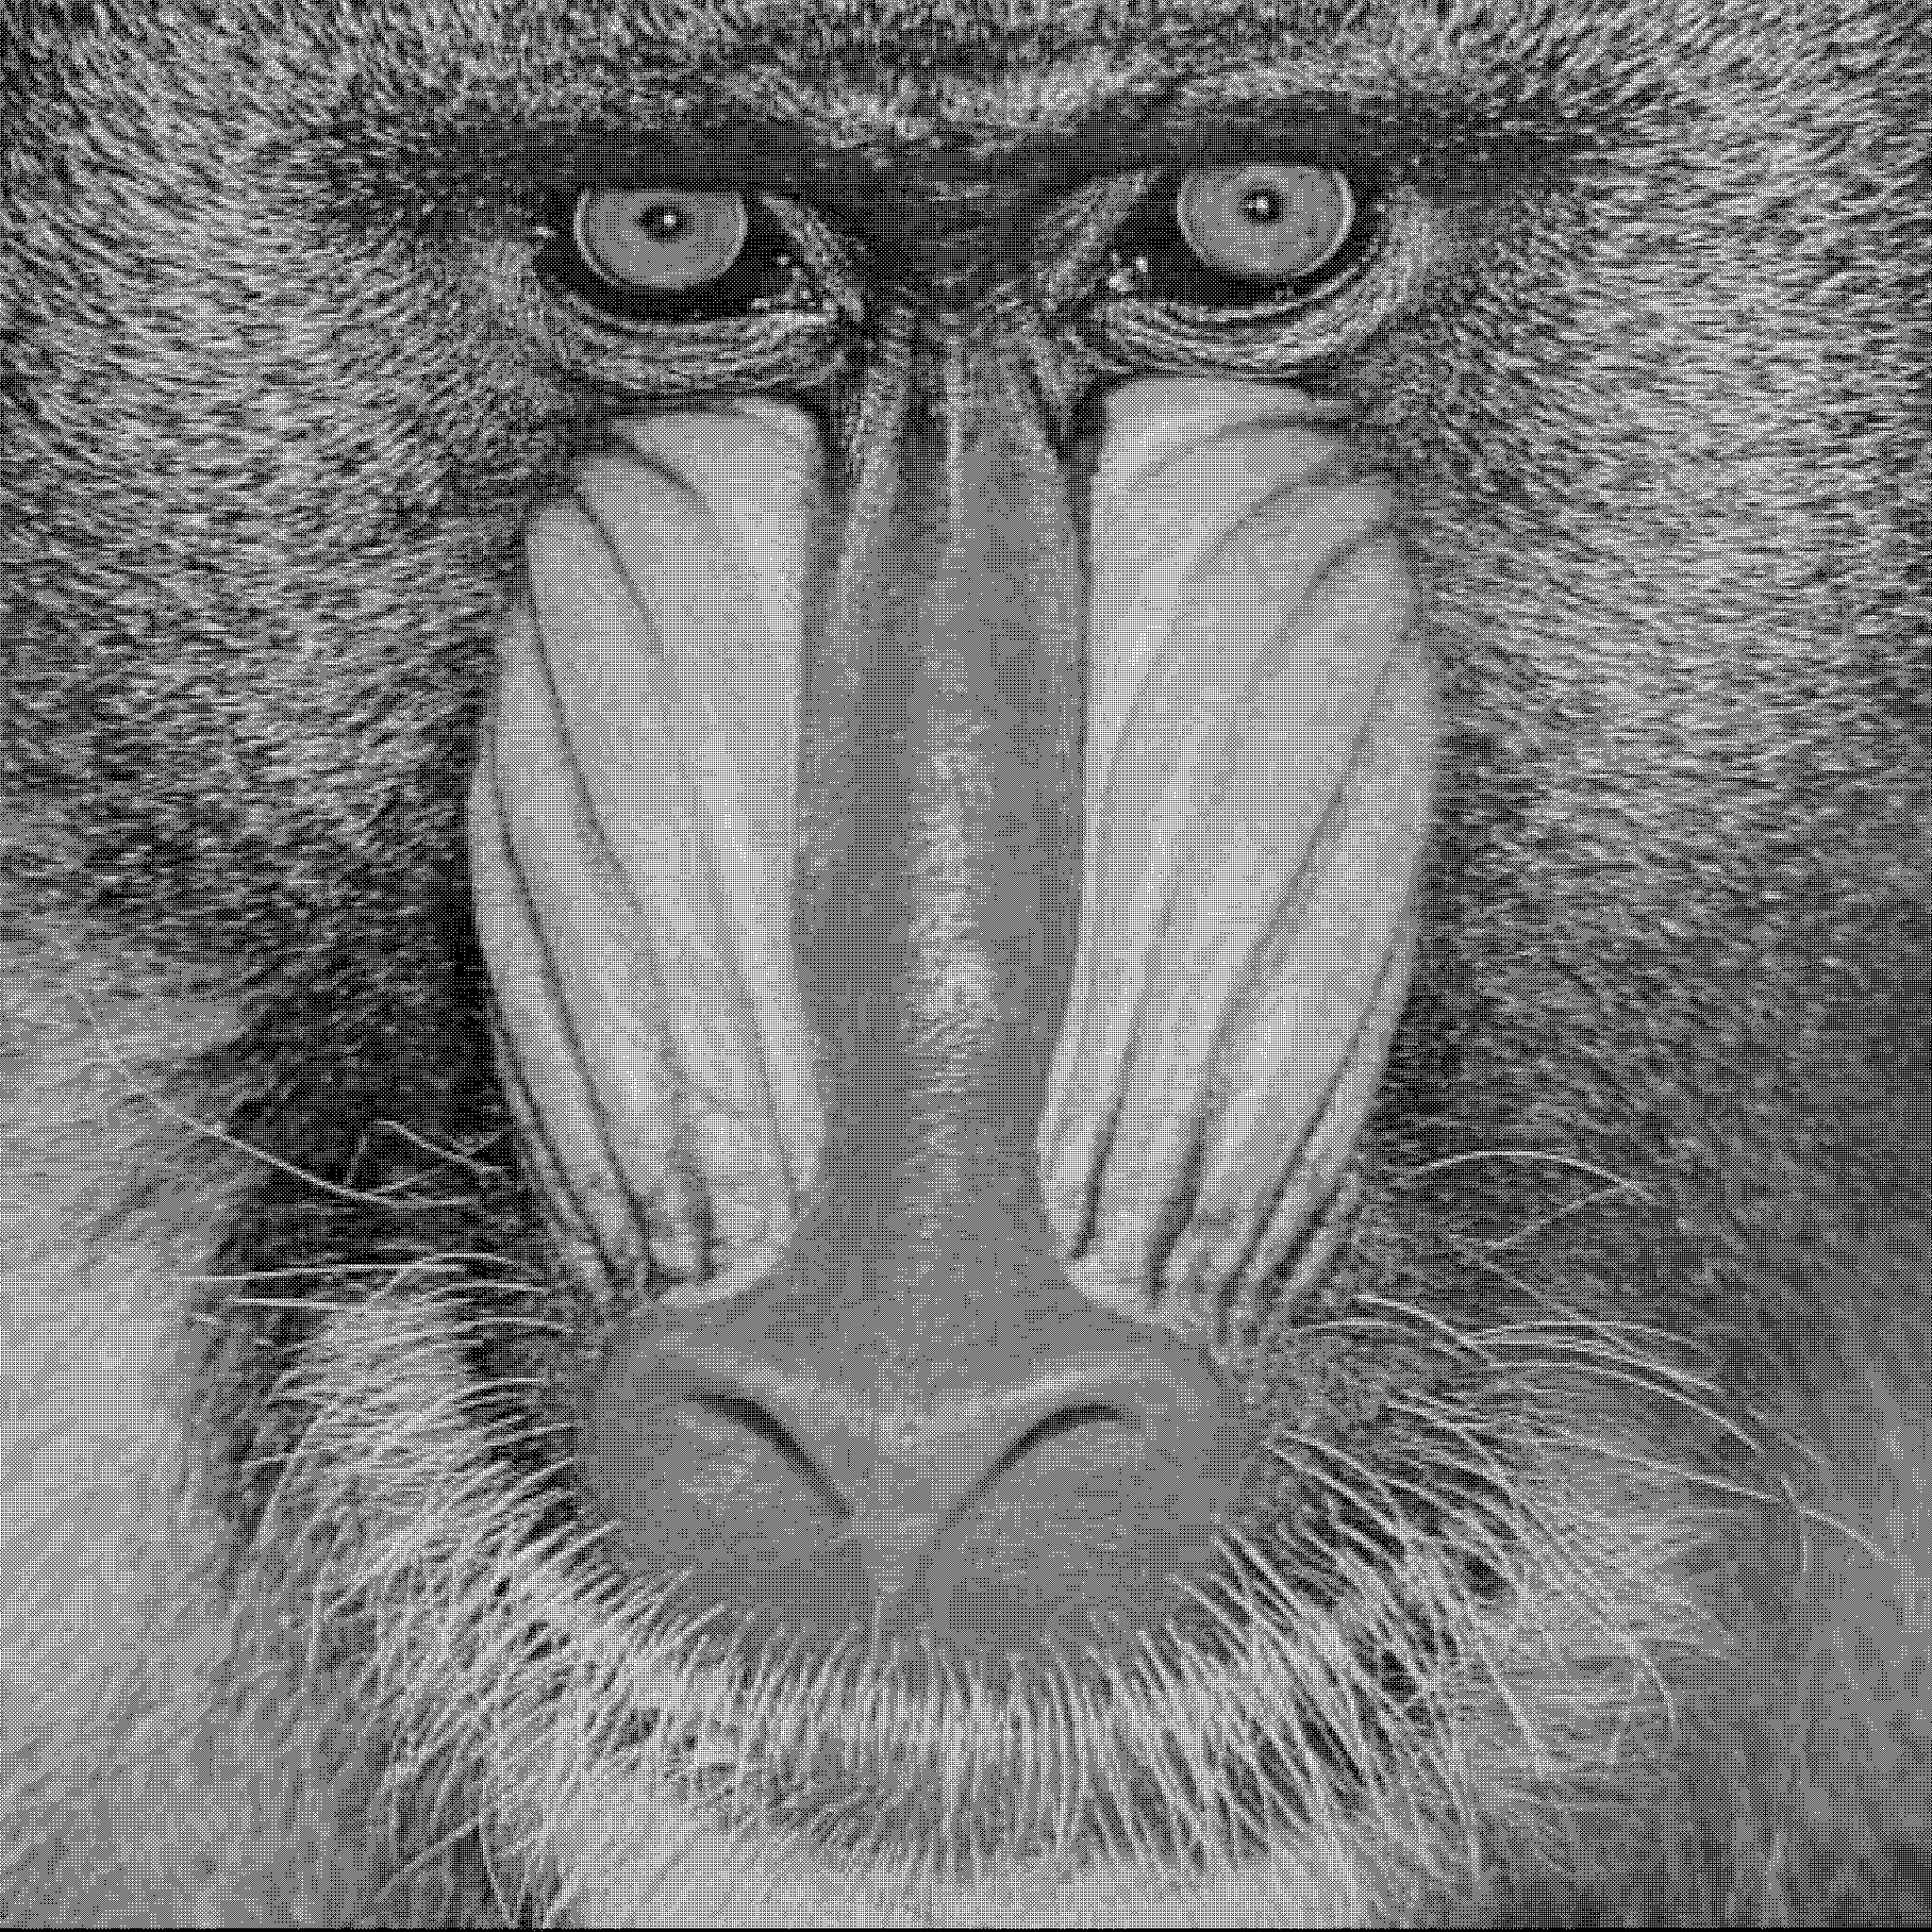
\includegraphics[height=4cm]{figures/baboon_m44.png}
\caption{Aplicação das máscaras $M_{3x3}$ e $M_{4x4}$, respectivamente, na imagem \textbf{baboon.pgm}.} \label{baboonm33m44}
\end{center}
\end{figure}

A Figura~\ref{baboonm33m44} apresenta os resultados da aplicação na imagem \textbf{baboon.pgm}, o qual o resultado da esquerda sofreu um aumento nas dimensões da imagem de $300\%$, pois isso está diretamente ligado ao tamanho da máscara. Como a máscara é $3x3$, a imagem resultando possui $3$ vezes mais \textit{pixels} na dimensão $x$ e $y$. A imagem resultante é formada também só por \textit{pixels} pretos e brancos, pois cada \textit{pixel} da imagem original resulta em ''um \textit{pixel}'' do tamanho da máscara com valores $0$ ou $255$, porém no final, as imagens são transformadas em binárias para que cada \textit{pixel} seja representado por um bit. A imagem que representa o resultado da aplicação da máscara $M_{4x4}$ (imagem da direita), possui dimensoes $4$ vezes maiores, por conta do tamanho da máscara. Como resutado visual, podemos observar que as imagens sofreram uma granularização dos \textit{pixels} de acordo com o tamanho da máscara, é possível observar pequenos quadrados, proporcionais ao tamanho da máscara, na imagem. Então, podemos constatar que quanto maior for a máscara, maior será a imagem resultante e menor será a percepção desses quadrados, se as imagens forem vistas com uma mesma dimensão final.

\begin{figure}[H]
\begin{center}
	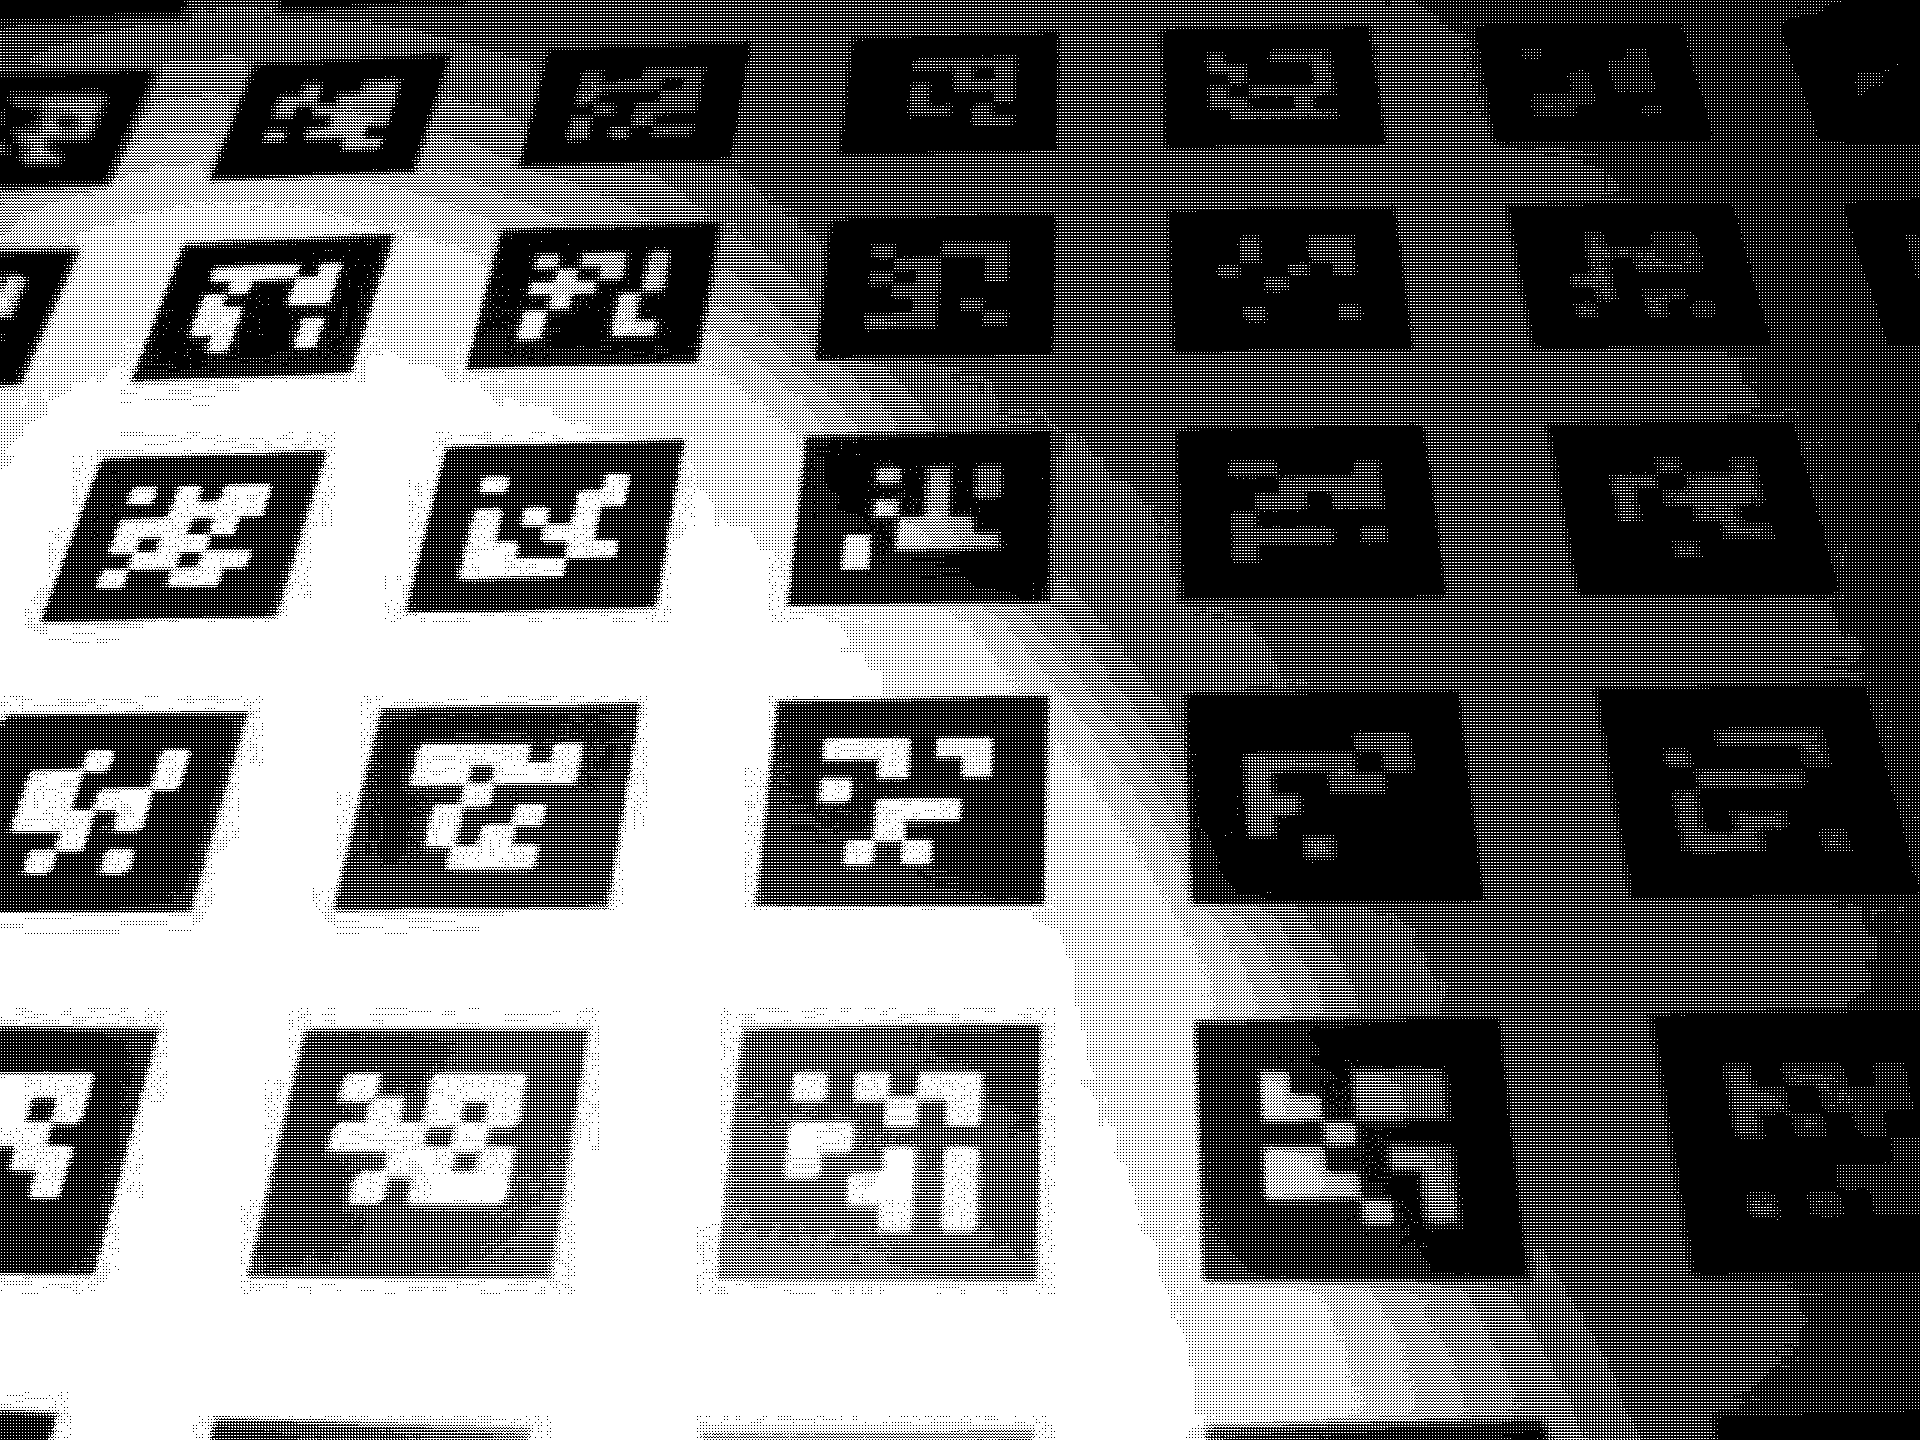
\includegraphics[height=3cm]{figures/fiducial_m33.png}
	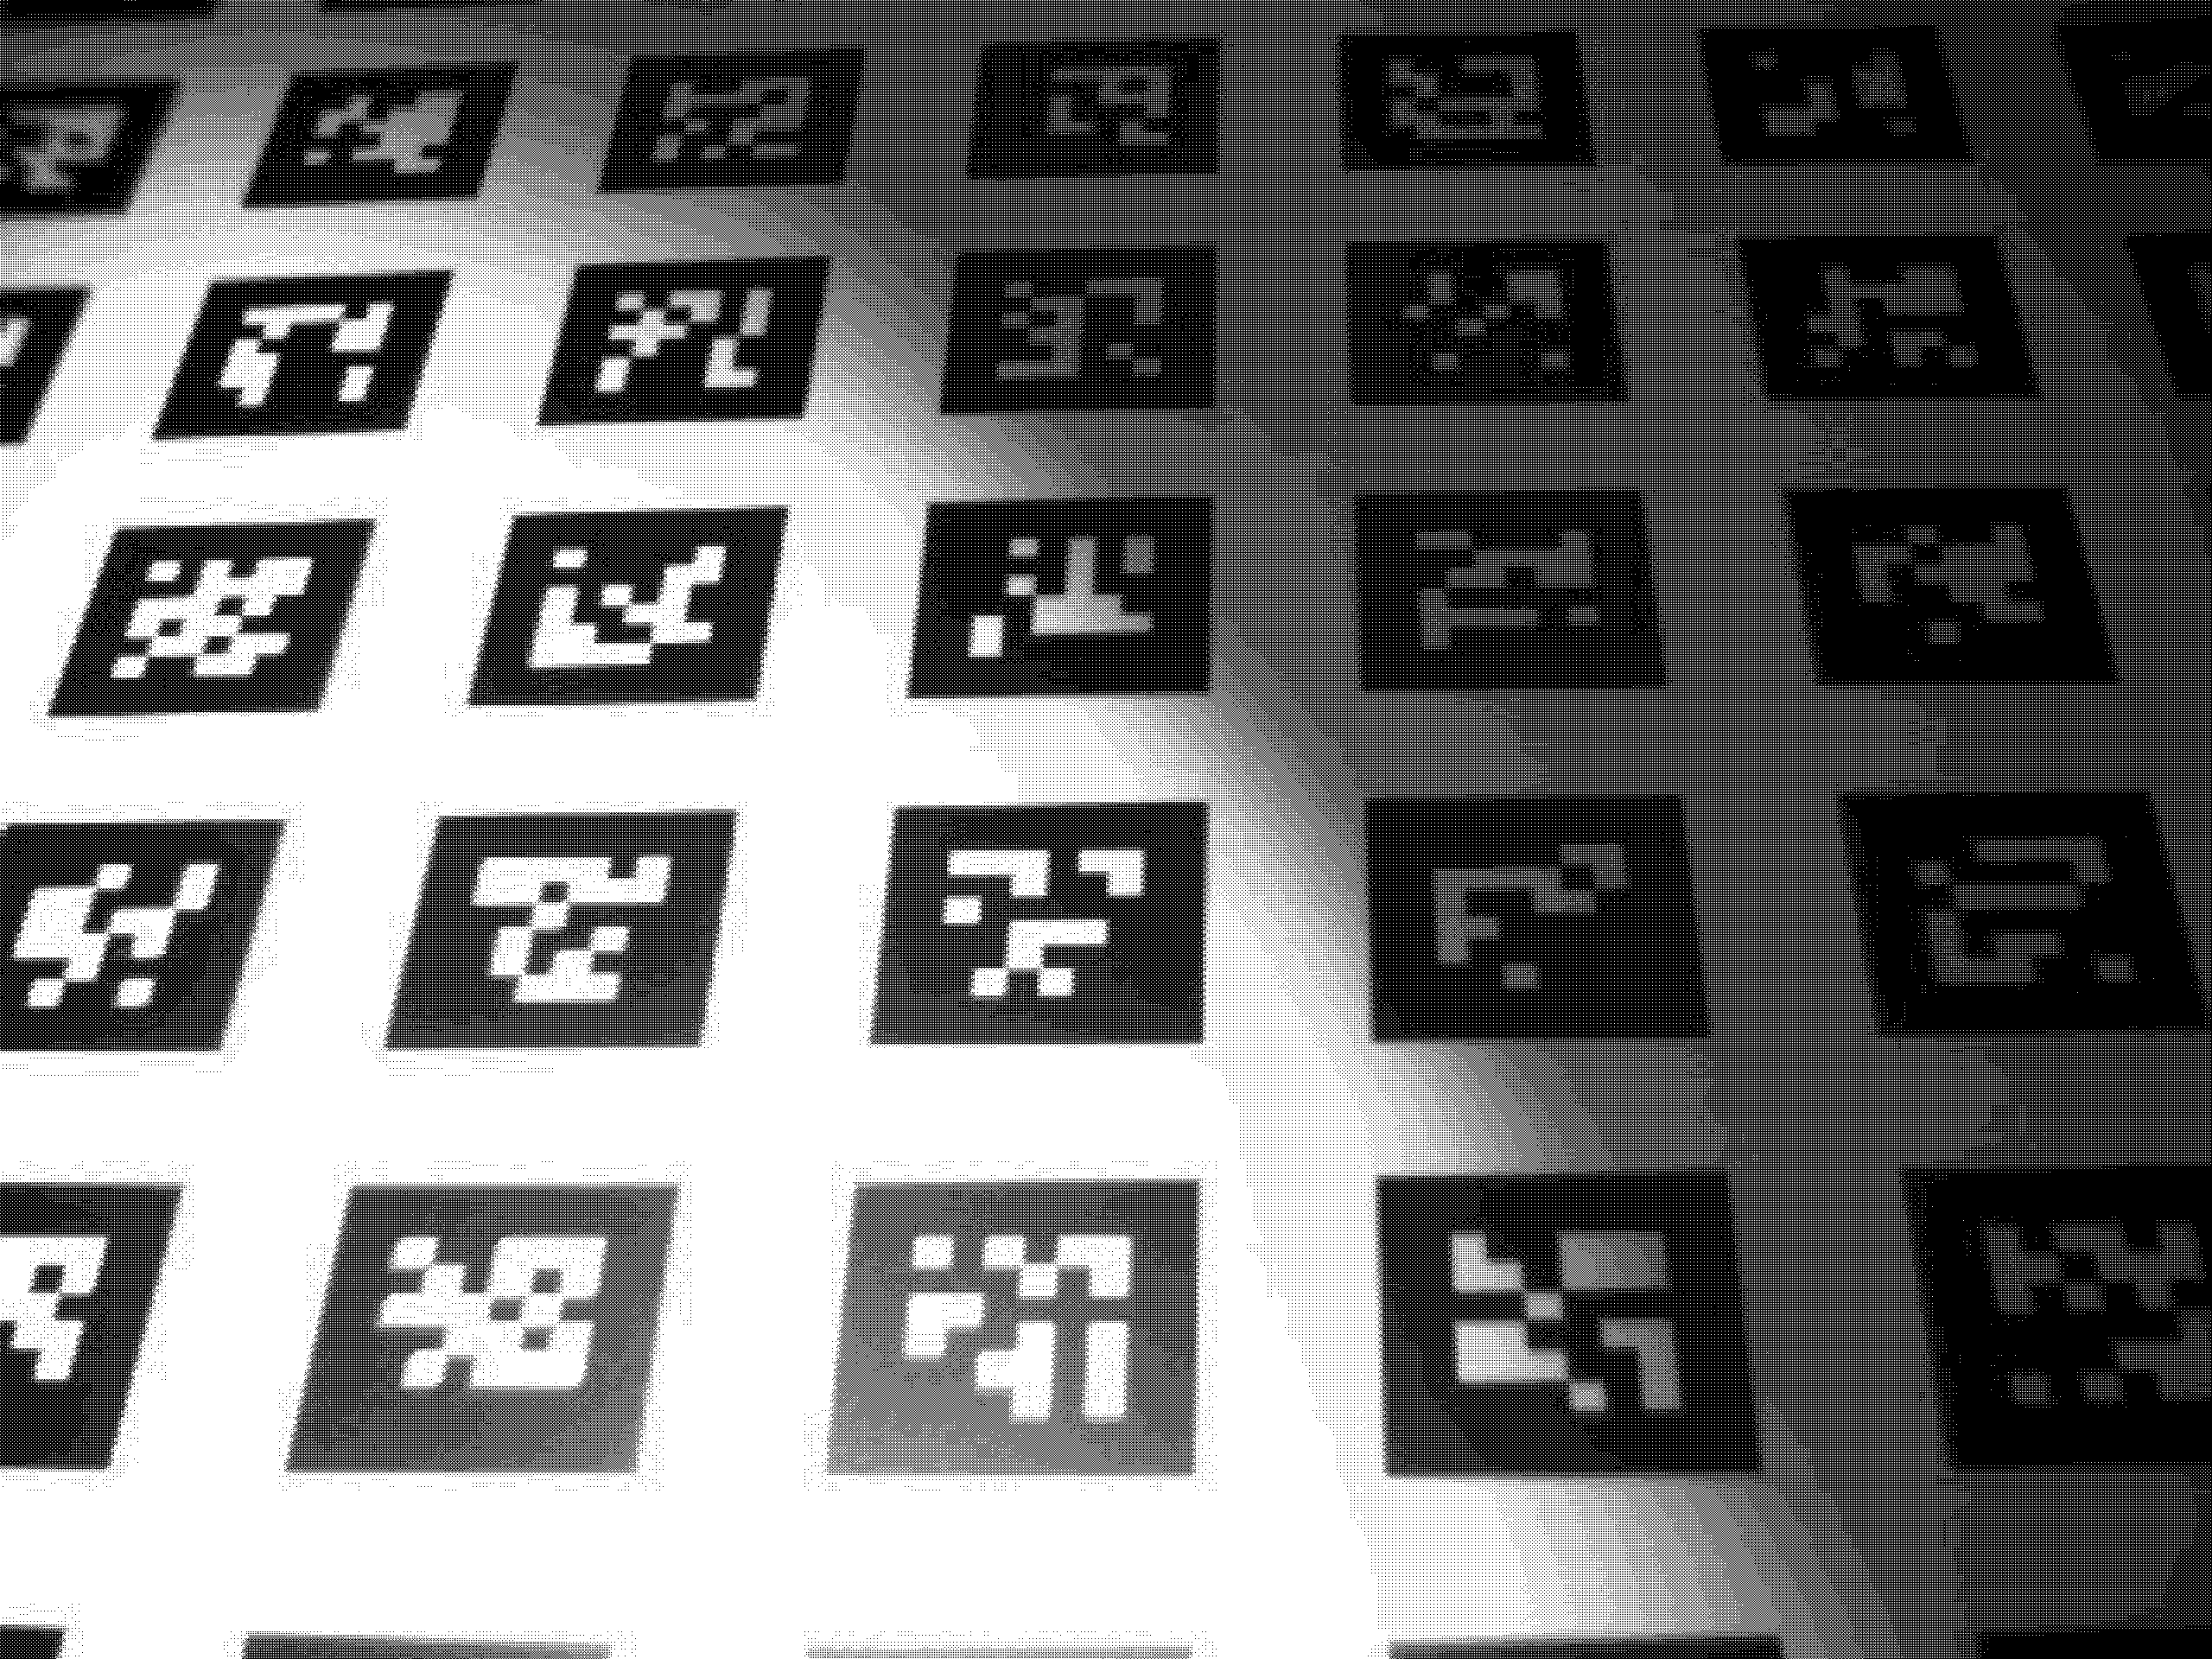
\includegraphics[height=3cm]{figures/fiducial_m44.png}
\caption{Aplicação das máscaras $M_{3x3}$ e $M_{4x4}$, respectivamente, na imagem \textbf{fiducial.pgm}.} \label{fiducialm33m44}
\end{center}
\end{figure}

Na Figura~\ref{fiducialm33m44}, podemos constatar que o tamanho das imagens foi alterado também de acordo com o tamanho das máscaras, e como essa imagem de entrada possui menos detalhes que a anterior, pode-se observar melhor a diferença entre a aplicação das duas máscaras, a qual a máscara $M_{4x4}$ torna a imagem resultante mais nítida que a aplicação com a máscara $M_{3x3}$.

\begin{figure}[H]
\begin{center}
	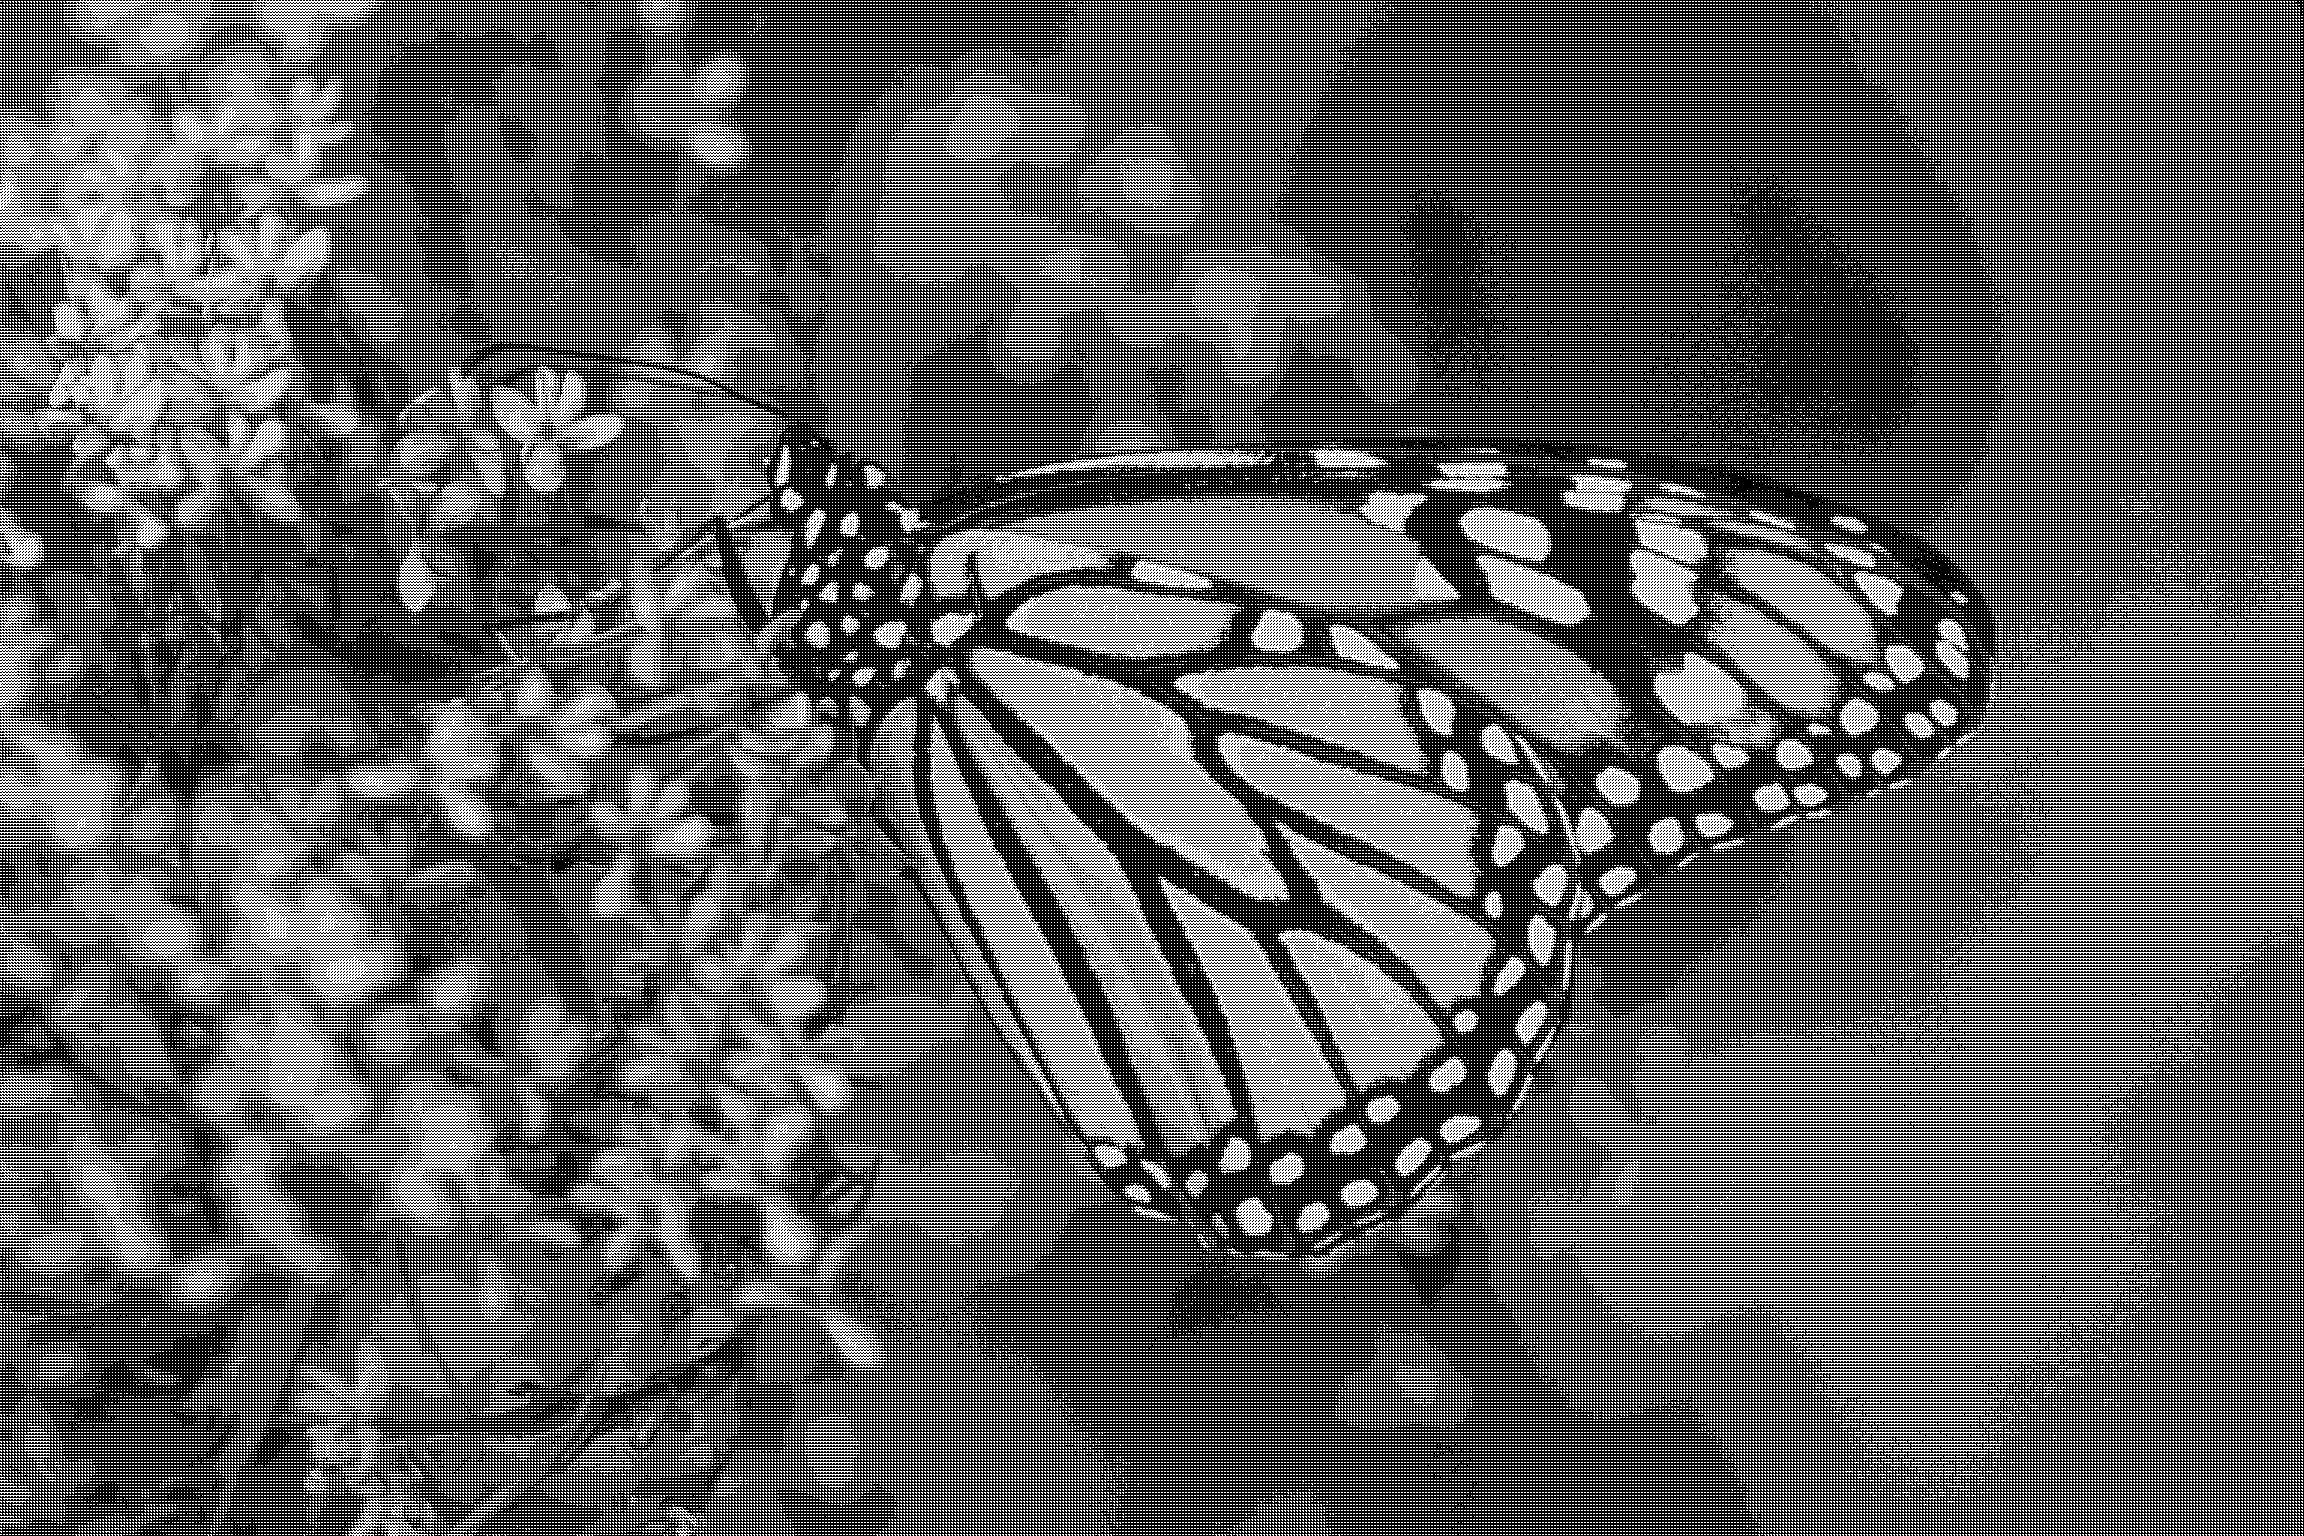
\includegraphics[height=3cm]{figures/monarch_m33.png}
	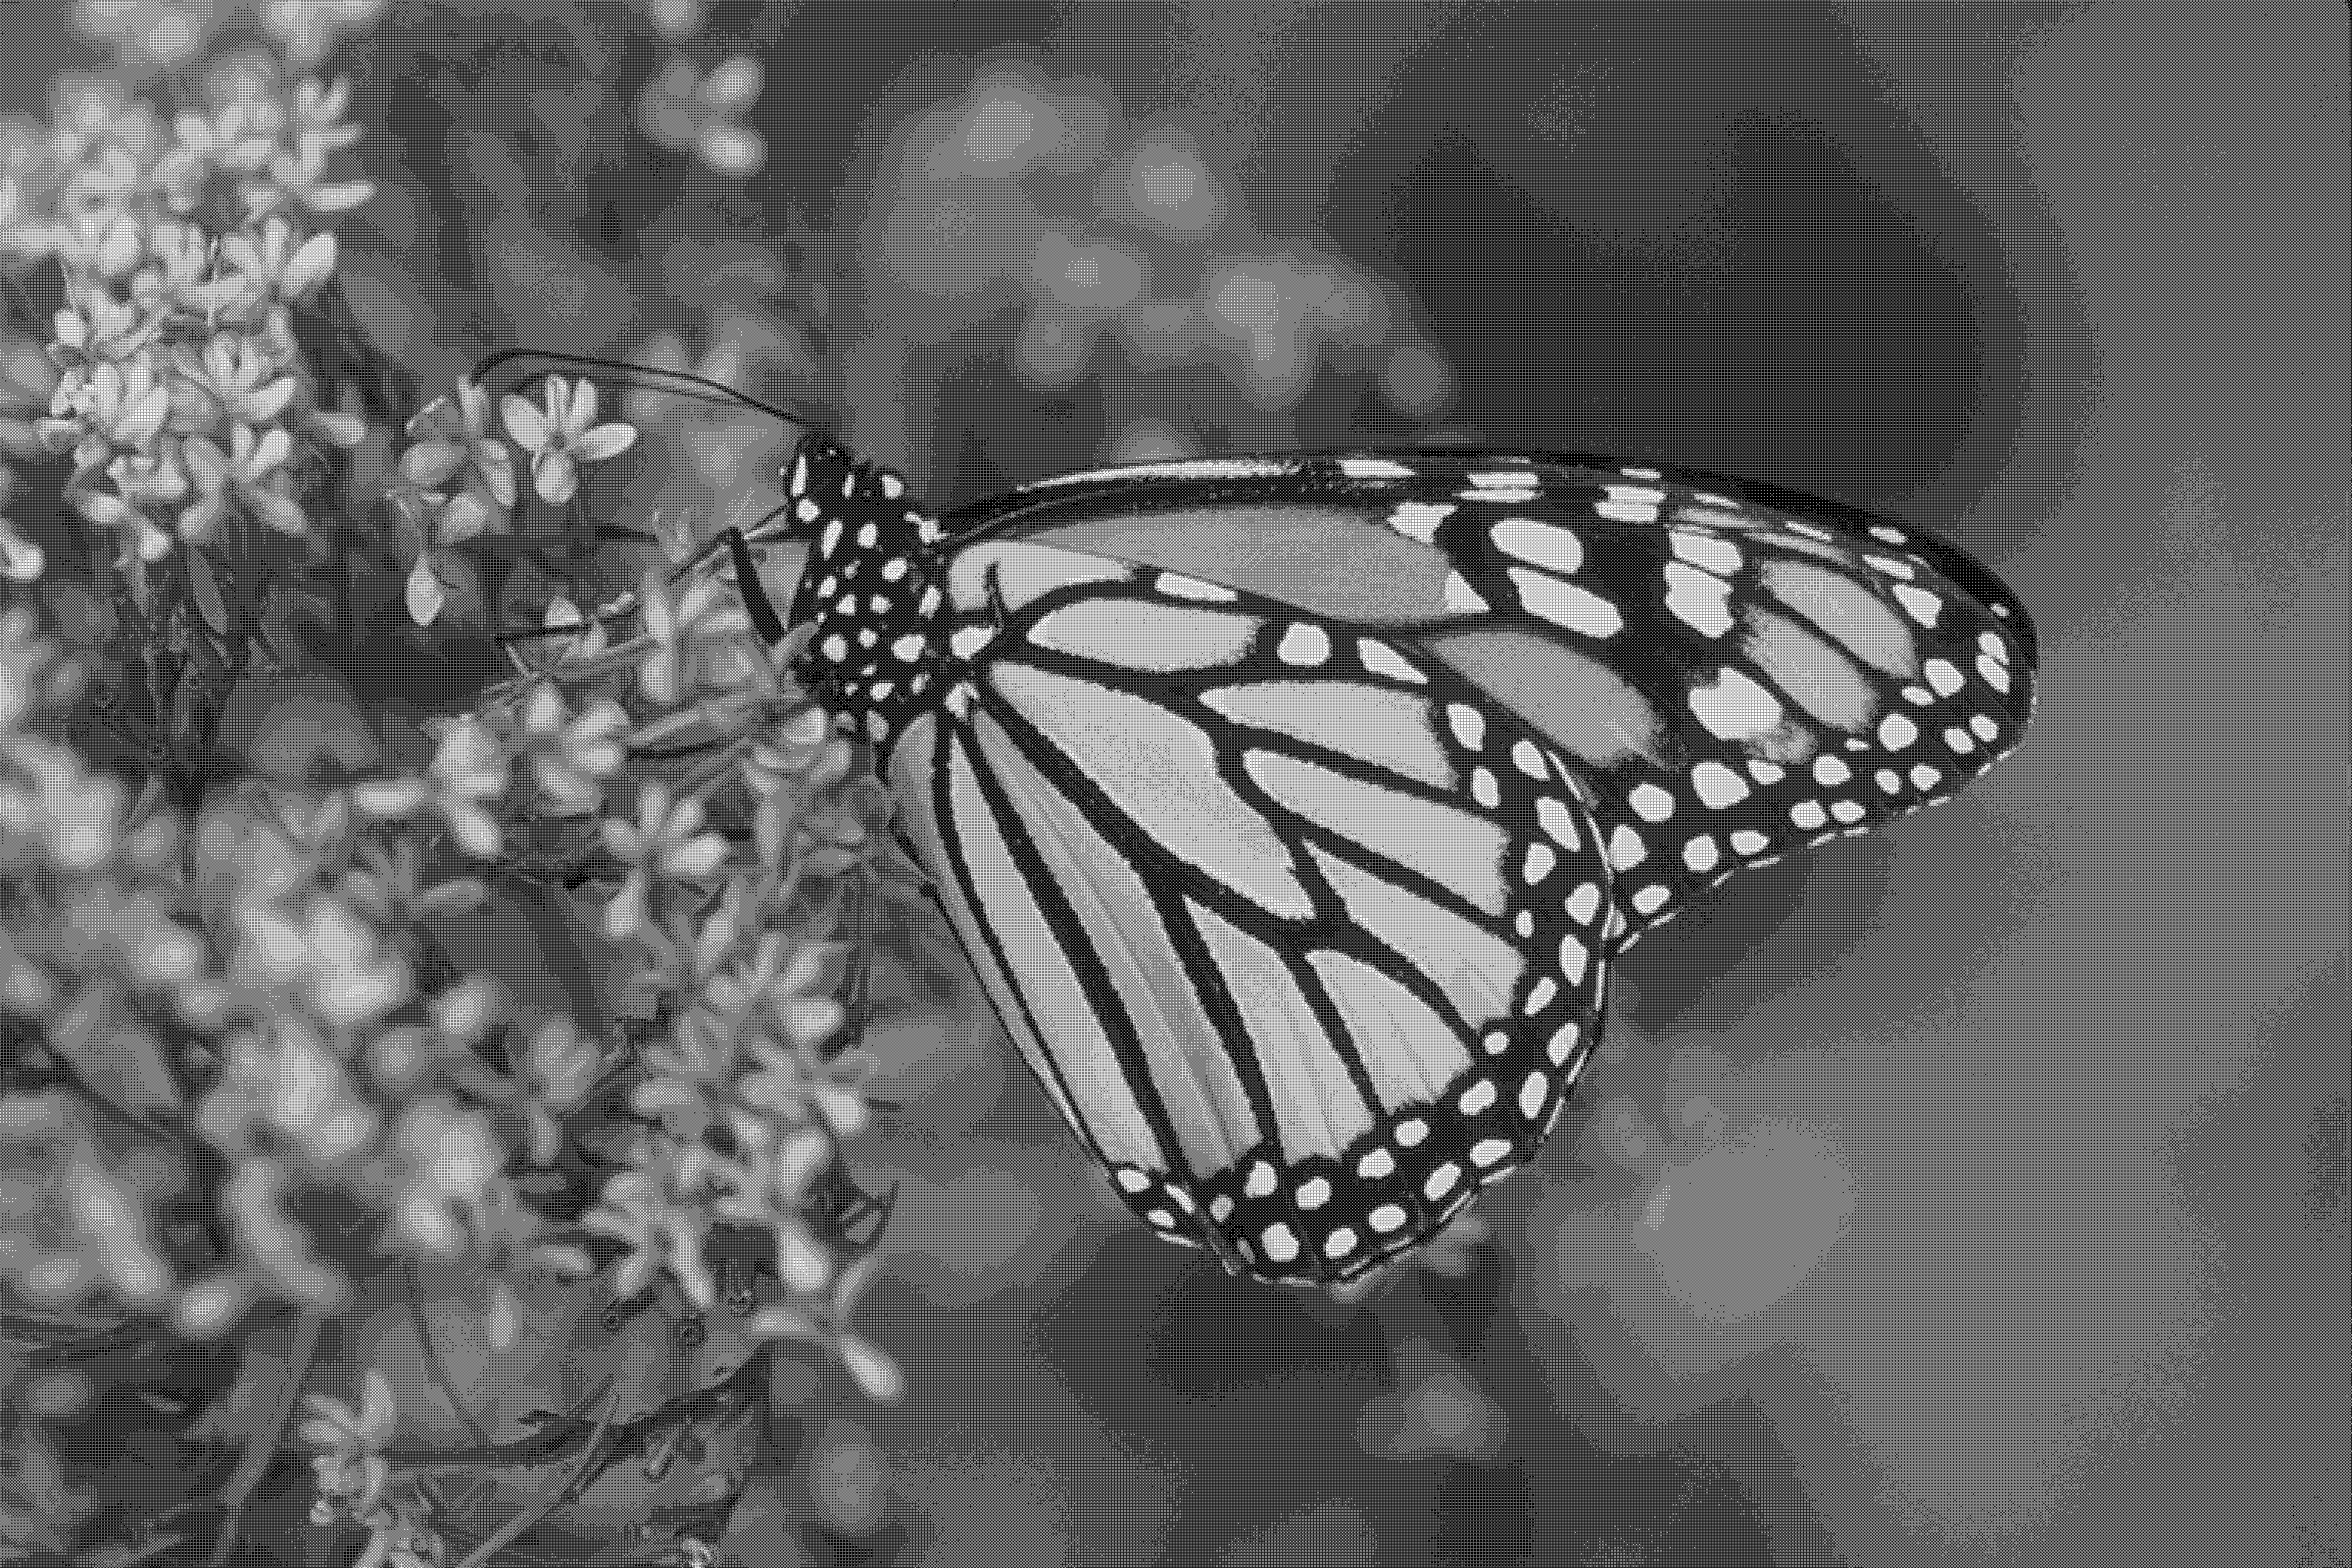
\includegraphics[height=3cm]{figures/monarch_m44.png}
\caption{Aplicação das máscaras $M_{3x3}$ e $M_{4x4}$, respectivamente, na imagem \textbf{monarch.pgm}.} \label{monarchm33m44}
\end{center}
\end{figure}

Na Figura~\ref{monarchm33m44}, podemos observar que algumas regiões sofreram um ''agrupamento de intensidades'' bem maior com a máscara $M_{3x3}$ do que com a máscara $M_{4x4}$, a qual torna a imagem resultante com maior diferenciação visual das regiões, tendo assim um resultado melhor que o da aplicação da máscara $M_{3x3}$.

Os resultados obtidos com a aplicação da técnica de pontilhado com difusão de erro (\textit{Floyd-Steinberg}) estão a seguir:

\begin{figure}[H]
\begin{center}
	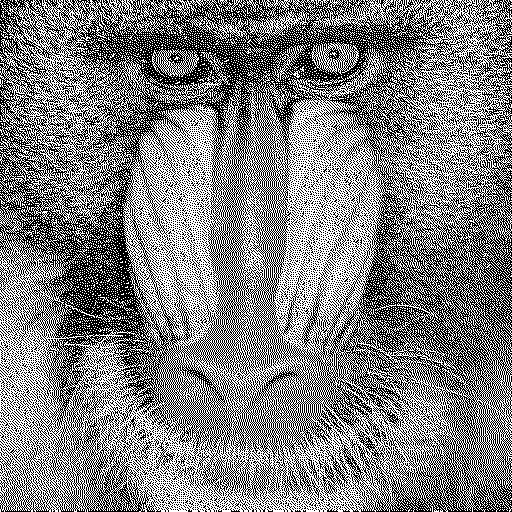
\includegraphics[height=4cm]{figures/baboon_floyd_order1.png}
	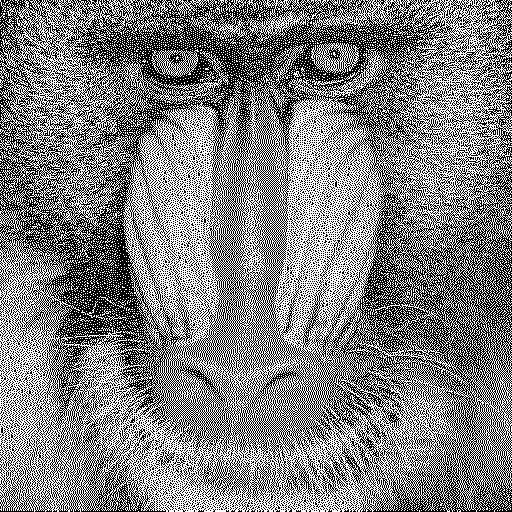
\includegraphics[height=4cm]{figures/baboon_floyd_order2.png}
\caption{Aplicação a técnica de pontilhado com difusão de erros percorrendo a imagem \textbf{baboon.pgm} das duas formas.} \label{baboonmfloyd}
\end{center}
\end{figure}

A Figura~\ref{baboonmfloyd} apresenta os resultados obtidos com a aplicação da técnica de pontilhado com difusão de erros, com duas formas de percorrer a imagem de entrada. As imagens resultantes não sofrem mudança nas suas dimensões, diferente da técnica anterior, e também são formadas apenas por \textit{pixels} pretos e brancos. Como a imagem \textbf{baboon.pgm} possui um alto nível de detalhes, não é possível observar uma diferença significativa entre as duas formas de difundir o erro de cada \textit{pixel}.

\begin{figure}[H]
\begin{center}
	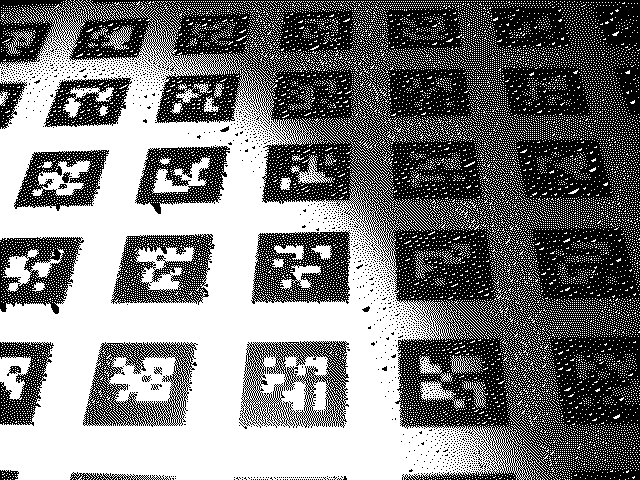
\includegraphics[height=3cm]{figures/fiducial_floyd_order1.png}
	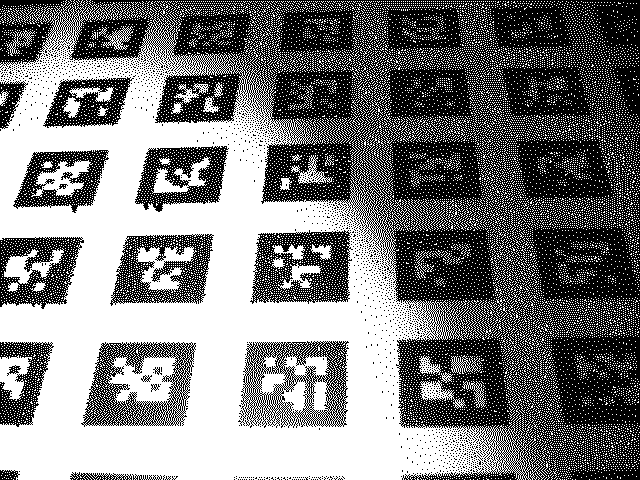
\includegraphics[height=3cm]{figures/fiducial_floyd_order2.png}
\caption{Aplicação a técnica de pontilhado com difusão de erros percorrendo a imagem \textbf{fiducial.pgm} das duas formas.} \label{fiducialfloyd}
\end{center}
\end{figure}

Na Figura~\ref{fiducialfloyd}, podemos observar que muitas regiões da primeira imagem possui algumas falhas, como conjuntos de \textit{pixels} pretos em locais que era para ter \textit{pixels} brancos, e vice-versa. Já na segunda imagem vemos que muitas das áreas defeituosas na primeira imagem estão consertadas aplicando a técnica de difusão de erro percorrendo de forma alternada, pois os erros são propagados nas direções esquerda-direita e direita-esquerda.

\begin{figure}[H]
\begin{center}
	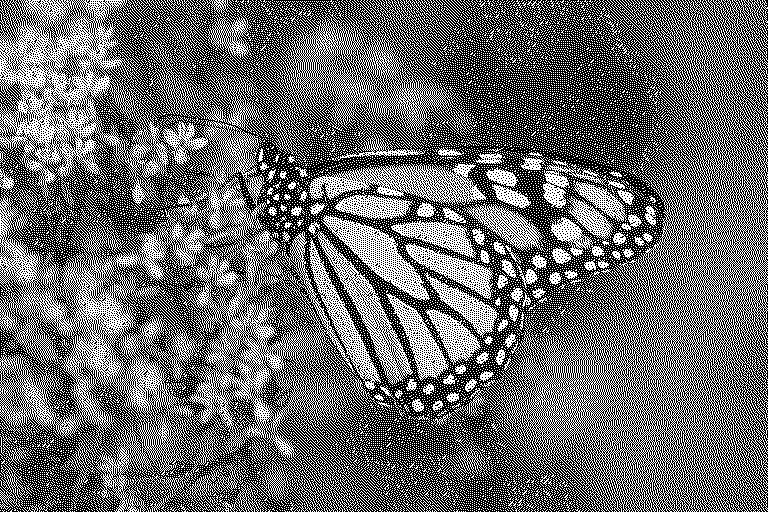
\includegraphics[height=3cm]{figures/monarch_floyd_order1.png}
	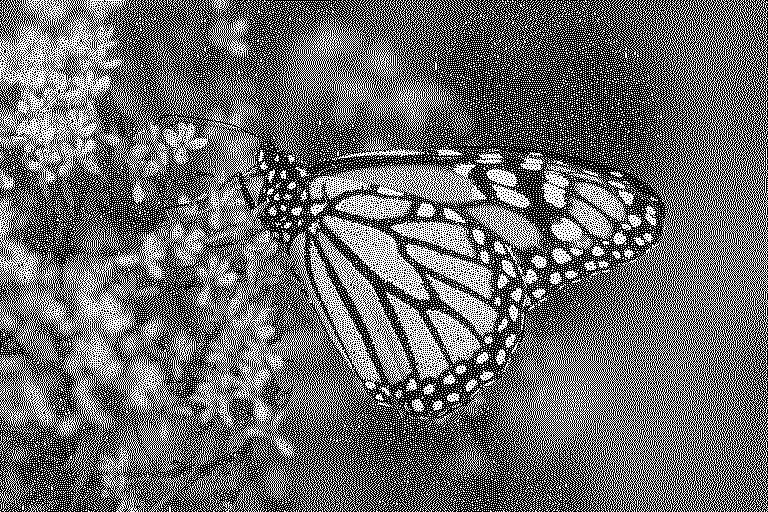
\includegraphics[height=3cm]{figures/monarch_floyd_order2.png}
\caption{Aplicação a técnica de pontilhado com difusão de erros percorrendo a imagem \textbf{monarch.pgm} das duas formas.} \label{monarchfloyd}
\end{center}
\end{figure}

Na Figura~\ref{monarchfloyd}, podemos observar que em conjuntos de \textit{pixels} que são limitantes de regiões com difentes intensidades, a aplicação da técnica percorrendo somente no sentido esquerda-direita, esses \textit{pixels} tendem a ficar mais visíveis, porém, percorrendo de maneira alternada, as regiões de fronteiras tendem a ficar menos abruptas.

Com esses experimentos, podemos destacar a aplicação da técnica de difusão de erros de maneiras alternada obteve melhor resultado do que difudindo o erro somente em um sentido.

%------------------------------------------------

\section{Conclusão}

Podemos concluir que os resultados obtidos com as aplicações das técnicas de pontilhado ordenado e pontilhado com difusão de erro foram satisfatórios quanto a especificação do trabalho e que a visualização prática da normalização da imagem, transformação para intensidade binária e transformações com pontilhados nas imagens consolida ainda mais os conceitos vistos em sala de aula.

%----------------------------------------------------------------------------------------
%	REFERENCE LIST
%----------------------------------------------------------------------------------------

\begin{thebibliography}{99} % Bibliography - this is intentionally simple in this template

\bibitem{b1} Welcome to opencv documentation! \href{https://docs.opencv.org/2.4/index.html}{https://docs.opencv.org/2.4/index.html} Acesso em: 04/05/2019.

\bibitem{b2} Pedrini, Hélio, and William Robson Schwartz. Análise de imagens digitais: princípios, algoritmos e aplicações. Thomson Learning, 2008.

\bibitem{b3} Matplotlib Version 3.0.3 \href{https://matplotlib.org/contents.html}{https://matplotlib.org/contents.html} Acesso em: 04/05/2019.

\bibitem{b4} SAWP, Dithering \href{http://www.sawp.com.br/blog/?p=940}{http://www.sawp.com.br/blog/?p=940} Acesso em: 04/05/2019.

\bibitem{b5} Digital Image Processing Using Python \href{https://ckpytsan.wordpress.com/2011/01/14/dithering-parte-iii-dithering-com-difusao-de-erro-e-o-algoritmo-de-floyd-steinberg/}{https://ckpytsan.wordpress.com/2011/01/14/dithering-parte-iii-dithering-com-difusao-de-erro-e-o-algoritmo-de-floyd-steinberg/} Acesso em: 04/05/2019.

\bibitem{b6} Wikipedia: Floyd–Steinberg dithering \href{https://en.wikipedia.org/wiki/Floyd-Steinber_dithering}{https://en.wikipedia.org/wiki/Floyd-Steinber_dithering} Acesso em: 04/05/2019.
 
\end{thebibliography}

%----------------------------------------------------------------------------------------

\end{document}
